\documentclass[11pt]{article}

\usepackage{a4wide}
\usepackage{amssymb}
\usepackage{stmaryrd}
\usepackage{proof}
\usepackage{amsmath}
\usepackage{listings}
\usepackage{graphicx}
\usepackage{cite}

\newcommand{\jStar}{{\sf jStar}}

\newcommand{\psto}{\mapsto}
\newcommand{\sem}[1]{[\!|#1 |\!] }
\newcommand{\rearr}{\mathsf{rearr}}
\newcommand{\FNames}{\mathit{FNames}}
\newcommand{\MNames}{\mathit{MNames}}
\newcommand{\CNames}{\mathit{CNames}}
\newcommand{\TNames}{\mathit{TNames}}
\newcommand{\NodeLL}{\mathit{NodeLL}}
\newcommand{\val}{\mathit{val}}
\newcommand{\intT}{\mathit{int}}
\newcommand{\next}{\mathit{next}}
\newcommand{\returnStm}{{\sf return}}
\newcommand{\invoke}{{\sf invoke}}
\newcommand{\sinvoke}{{\sf sinvoke}}
\newcommand{\jsr}{{\sf jsr}}
\newcommand{\init}{{\sf init}}
\newcommand{\emp}{{\sf emp}}
\newcommand{\TT}{{\sf true}}
\newcommand{\FF}{{\sf false}}
\newcommand{\void}{\mathit{void}}
\newcommand{\spec}{{\sf spec}}
\newcommand{\sspec}{{\sf sspec}}
\newcommand{\new}{{\sf new}}
\newcommand{\ra}{\longrightarrow}
\newcommand{\pto}{\mapsto}
\newcommand{\ret}{\mathit{ret}}
\newcommand{\refe}[4]{#1.\langle #2{:} \; #3 \ #4 \rangle}
\newcommand{\signature}[3]{\langle #1{:} \; #2 \ #3 \rangle}
\newcommand{\Sig}{\mathit{Sig}}
\newcommand{\Specs}{\mathit{Specs}}
\newcommand{\Heaps}{\mathit{Heaps}}
\newcommand{\Val}{\mathit{Val}}
\newcommand{\Powerset}{{\cal P}}
\newcommand{\lseg}{{\sf lseg}} 
\newcommand{\nil}{{\sf nil}} 
\newcommand{\junk}{{\sf junk}} 
\newcommand{\Var}{\mathit{Var}} 

%\newcommand{\ex}[1]{\mathord{\_\!\_#1}}
\newcommand{\ex}[1]{\mathord{\hat{#1}}}

% Definition for specifications
\newcommand{\define}{\mathbf{define} \ }
\newcommand{\content}[1]{\{\text{content=} \, #1 \}}
\newcommand{\true}{\mathbf{true}}
\newcommand{\symbolicheap}[2]{#1 \mid #2}
\newcommand{\this}{\mathbf{this}}
\newcommand{\return}{\mathbf{return}}
\newcommand{\parameter}{\mathbf{param0}}
\newcommand{\contentOld}[2]{\{\text{content=} \, #1; \  \text{old=} \, #2 \}}
\newcommand{\type}{\mbox{type}}
\newcommand{\Visitor}{\mathit{Visitor}}
\newcommand{\Ast}{\mathit{Ast}}
\newcommand{\Visited}{\mathit{Visited}}
\newcommand{\context}[1]{\{\text{context=} \, #1 \}}
\newcommand{\contentCA}[3]{\{\text{content=} \, #1; \  \text{context=} \, #2; \ \text{ast=} \, #3 \}}
\newcommand{\export}{\mathbf{export}}
\newcommand{\const}{\mathit{const}}
\newcommand{\plus}{\mathit{plus}}
\newcommand{\lft}{\mathit{left}}
\newcommand{\rgt}{\mathit{right}}
\newcommand{\summ}{\mathit{sum}}
\newcommand{\union}{\mathit{union}}
\newcommand{\amount}{\mathit{amount}}
\newcommand{\rz}{\mathit{rz}}
\newcommand{\isZero}{\mathit{isZero}}
\newcommand{\isChanged}{\mathit{isChanged}}
\newcommand{\newl}{\mathit{newl}}
\newcommand{\false}{\mathbf{false}}
\newcommand{\zero}{\mathbf{zero}}
\newcommand{\DBPool}{\mathit{D\!B\!Pool}}
\newcommand{\DBConnection}{\mathit{D\!B\!Connection}}
\newcommand{\connection}[1]{\{\text{connection=} \, #1 \}}
\newcommand{\sql}{\mathit{sql}}
\newcommand{\url}{\mathit{url}}
\newcommand{\user}{\mathit{user}}
\newcommand{\password}{\mathit{password}}
\newcommand{\conns}{\mathit{conns}}
\newcommand{\LinkedList}{\mathit{LinkedList}}
\newcommand{\DBSet}{\mathit{D\!B\!Set}}
\newcommand{\setof}{\mathit{setof}}
\newcommand{\handle}[2]{\{\text{handle=} \, #1; \  \text{type=} \, #2 \}}
\newcommand{\ResourceFactory}{\mathit{ResourceFactory}}
\newcommand{\Resource}{\mathit{Resource}}
\newcommand{\factory}[2]{\{\text{factory=} \, #1; \  \text{type=} \, #2 \}}
\newcommand{\ResPool}{\mathit{ResPool}}
\newcommand{\resources}{\mathit{resources}}
\newcommand{\rf}{\mathit{rf}}
%\newcommand{\ResourceFactory}{\mathit{ResourceFactory}}
\newcommand{\IterRes}{\mathit{IterRes}}
\newcommand{\Subject}{\mathit{Subject}}
\newcommand{\ObsSet}{\mathit{ObsSet}}
\newcommand{\SubjectObs}{\mathit{SubjectObs}}
\newcommand{\observers}{\mathit{observers}}
\newcommand{\listIT}{\mathit{list}}
\newcommand{\SubjectData}{\mathit{SubjectData}}
\newcommand{\SubjectInternal}{\mathit{SubjectInternal}}
\newcommand{\obsVals}[2]{\{\text{obs=} \, #1; \  \text{vals=} \, #2 \}}
\newcommand{\obs}[1]{\{\text{obs=} \, #1 \}}
\newcommand{\vals}[1]{\{\text{vals=} \, #1 \}}
\newcommand{\valsSubject}[2]{\{\text{vals=} \, #1; \  \text{subject=} \, #2 \}}
\newcommand{\dollar}{\mbox{\$}}
\newcommand{\Observer}{\mathit{Observer}}
\newcommand{\add}{\mathit{add}}
\newcommand{\emptyP}{\mathit{empty}}




\newtheorem{thm}{Theorem}
\newtheorem{defn}{Definition}
\newtheorem{lemma}{Lemma}
\newtheorem{example}{Example}
\newtheorem{notation}{Notation}

\newcommand{\field}[3]{\textrm{#1}.\textrm{#2} \mapsto \textrm{#3}}




\lstset{language=Java,framesep=5pt,columns=fullflexible,basicstyle=\small,
 stringstyle=\ttfamily,
 showstringspaces=true,
 mathescape=true,
 deletekeywords={const},
 morekeywords={ensures,requires,inherit,andalso,define,as,dynamic,export,rule,rewrite},
 literate=
           {@}{$\$$}1
           {/\\}{$\land\ $}2
           {|-}{$\vdash\ $}2
           {|->}{$\mapsto\ $}2
           {@this:}{\textbf{this}}4
           {inherited\ with\ type}{\textbf{inherited with type}}4
           {@parameter0:}{\textbf{param0}}6
           {@parameter1:}{\textbf{param1}}6
           {@parameter2:}{\textbf{param2}}6
           {@return:}{\textbf{return}}6
           {-*}{$\mathbin{-\!*\,}$}6
,}
\def\J{\lstinline}
\newcommand{\JS}[1]{$\mathit{#1}$}


%\renewcommand{\jStar}{\raisebox{-.2em}{
\includegraphics[height=1em]{logo.pdf}}}
\newcommand{\jStarlogo}{\raisebox{-.2em}{
\includegraphics[height=1em]{logo.pdf}}}
%\newcommand{\jStarPlain}{jStar}
\newcommand{\jStarPlain}{\jStar}
\newcommand{\jStarQED}{\hfill \jStarlogo}


\newcommand{\mattcomment}[1]{
\begin{center}
\fbox{
\begin{minipage}{3.0in}
{\bf Matt's comment:} {\it #1}
\end{minipage}
}
\end{center}
}

\newcommand{\dinocomment}[1]{
\begin{center}
\fbox{
\begin{minipage}{3.0in}
{\bf Dino's comment:} {\it #1}
\end{minipage}
}
\end{center}
}

\begin{document}
\title{\bf How to Verify Java Program with \jStar: a  Tutorial \\[2ex]
\jStarlogo \qquad  \jStarlogo  \qquad \jStarlogo }

\author{{\sc Dino Distefano} \\
Queen Mary University of London, UK \\ 
{\tt ddino@dcs.qmul.ac.uk} 
\and 
{\sc Matthew J. Parkinson} \\
University of Cambridge, UK \\ 
{\tt Matthew.Parkinson@cl.cam.ac.uk}}

\maketitle

\begin{abstract}
  In this tutorial we describe how to use the tool \jStar \ to verify
  Java programs. The document is meant to be an informal and basic introduction to
  \jStar \ and many of the key notions behind this tool. 
  
  This is an evolving document, we hope to improve it along with the improvement of the tool.
\end{abstract}

\section{Introduction}
\jStar~\cite{jstar} is an automatic verification tool based on
separation logic aiming at object-oriented programs written in
Java. \jStar \ integrates theorem proving and abstract interpretation
techniques. The user is required to provide specifications of pre/post
conditions whereas loop invariants are synthesized  automatically,
minimizing the burden of verification.  \jStar \ uses succinct
separation logic specification therefore pre/post specs in this language are often 
simpler than what would be in other formalisms.

\jStar \ aims at those applications which present challenging problems
for the other verification tools for object-oriented
programs~\cite{jml,jmltool, spec, DHHR05,DLR06, chin08}.
Example of key challenges in verifying object-oriented programs are:
\begin{description}
\item [Properties across multiple objects] where one needs to be able
  to express properties about several interacting objects from many
  different classes.

\item [Call-backs] Methods often make calls that in turn will call the
  original object. This schema can cause great difficulty when one
  tries to verify it using class/object invariant based approaches.

\item [Modular verification] Verification must deal with a single
  class in isolation.  Adding new classes cannot invalidate the
  verification of pre-existing classes, and changing implementations
  while preserving specification should only require the re-verification
  of the changed code.
\end{description}

There are two key technologies undelying \jStar: the modular
verification technique of {\em abstract predicat families} defined by
Parkinson and Bierman \cite{Parkinson:popl05,PB:popl08} and the abstraction
techniques developed for separation logic developed by
Distefano {\em et al}~\cite{DOY:tacas06}.


\section{Basics}
\label{sec:basics}
\jStar's internal structure is depicted in
Figure~\ref{fig:architecture}.  It is composed by two main
components: a theorem prover and the symbolic execution module. The
prover is called by the symbolic execution during the verification
process to decide implications.  The symbolic execution module is
responsible for the fixed point computation of invariants.

\jStar \ accepts programs written in Jimple which is one of the Soot
toolkit intermediate representations~\cite{vall99soot} designed to
analyze Java programs. We use Soot for parsing Java into
Jimple, the latter is then parsed by \jStar \ into its internal data
structures. \jStar \ is implemented in OCaml.
%
\begin{figure}[t]
  \centering
  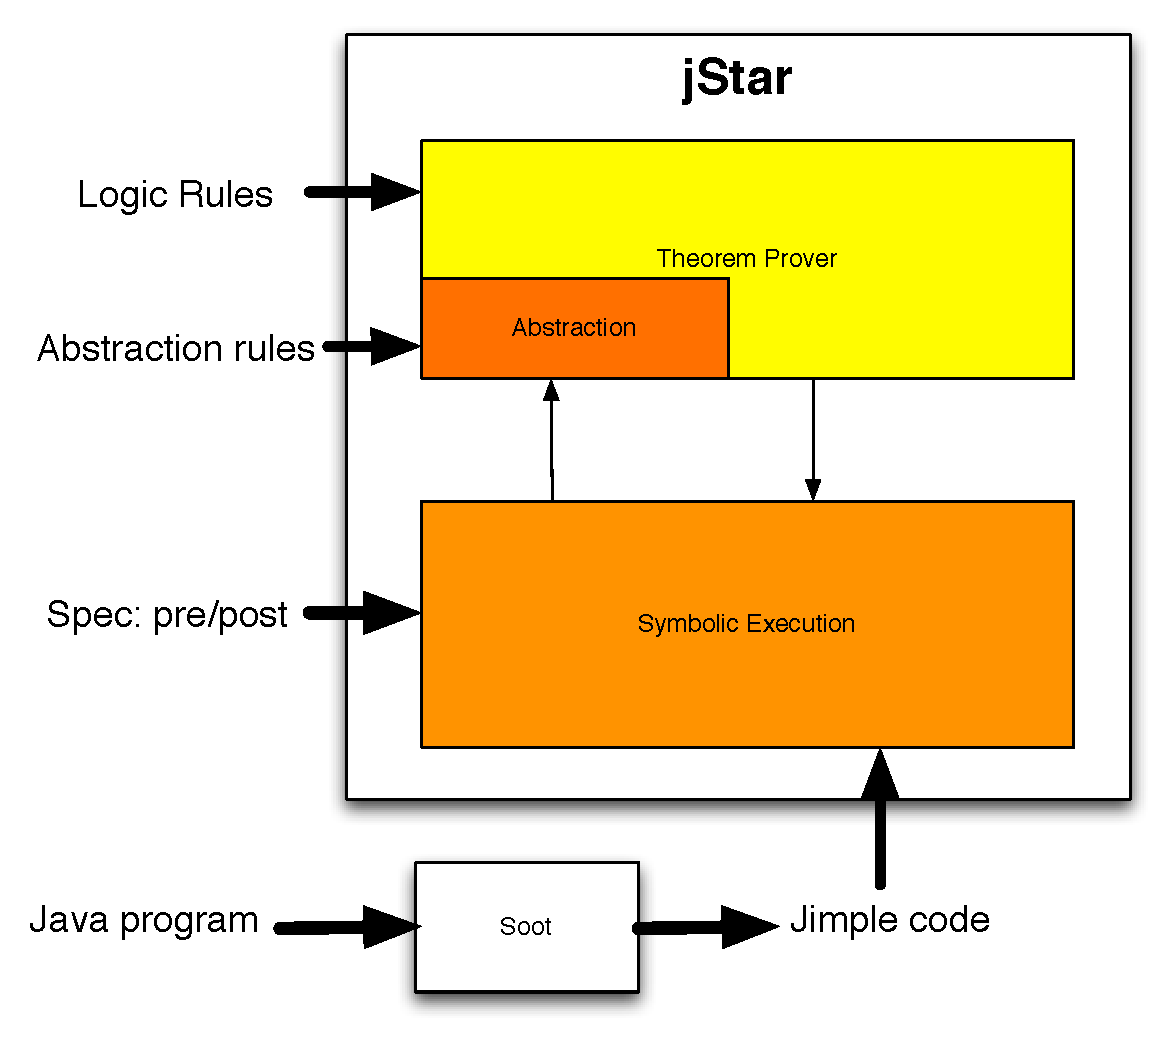
\includegraphics[width=2.9in]{architecture2}
  \caption[\jStarPlain\ architecture]{\jStar\ architecture}
  \label{fig:architecture}
\end{figure}
%
Other input files used by \jStar \ for the verification of a Java
program are:
\begin{description}
\item[Pre/post condition specifications.]  The user needs to specify
  pre and postconditions of the program's methods as well as the
  specification of the methods it calls. 

  Details on pre/postcondition specifications are discussed in
  Section~\ref{sec:pre/post}.
\item[Logic rules.]  In this file the user specifies the logical
  theory which is used by the theorem prover to decide entailment
  and other kinds of implications. The theory is specified by logical
  rules.  

  Details on logic rules are discussed in Section~\ref{sec:logic-rules}.
\item[Abstraction rules.]  This file defines the abstraction function
  used to ensure convergence in the fixed-point computation of
  loop-invariants. The abstraction function is defined by means of
  abstraction rules that are an extension of the logical rules. 
  
  Details on abstraction rules are discussed in
  Section~\ref{sec:abstraction-rules}.
\end{description}

\newcommand{\linkedlist}{\texttt{LinkedList.java} }
\subsection{Let's start}

\subsection{Let's start}
To run  \jStar \ on a Java program we need first to compile it in the
Jimple intermediated language. To do that the Soot~\cite{vall99soot} package
should be already installed and correctly working in your system. Consider the
\linkedlist \ program in Figure~\ref{tab:linkedlist}. Soot works on
bytecode therefore we first  compile it to produce the binary {\tt LinkedList.class}
with the command
\begin{verbatim}
 javac LinkedList.java
\end{verbatim}
And then run Soot to produce the jumple version of our program:
\begin{verbatim}
java soot.Main LinkedList -f J -d .
\end{verbatim}
At this point the file {\tt LinkedList.jimple} should be in the
current directory. To run \jStar \ on the file {\tt LinkedList.jimple}
using the logical rules contained in {\tt LinkedList.logic}, the
abstraction rules in {\tt LinkedList.abs} and the specification rules
in {\tt LinkedList.specs} simply type the command
\begin{verbatim}
jstar -l LinkedList.logic -a LinkedList.abs -s LinkedList.specs -f LinkedList.jimple
\end{verbatim}
Here we are using some of the command-line options available:\footnote{For 
the complete list of options, run {\tt jstar -help}.} 
\begin{description}
\item[-l] specifies the file containing the {\em logic rules} that
  \jStar \ needs to use in this run of the verification.
\item[-a] specifies the file containing the {\em abstraction rules}.
\item[-s] specifies the file containing the pre/post specifications of the methods in the program.
\item[-f] specifies the jimple translation of the program we want to
  verify.
\end{description}
\jStar \ should then reports that all methods have been verified (meening
that the \linkedlist \ meets the specifications defined in {\tt
  LinkedList.specs}), or reports an error (indicating which methods
could not be verified), or diverges (in case the abstraction function
is not strong enough to ensure the termination of the invariant
computation).
%
\begin{figure}[t]
  \centering
  \begin{tabular}{l|l}
    \begin{lstlisting}
class LinkedList
{
    private NodeLL head ;
    private NodeLL tail ;
    /* head == tail == null -> empty list */

    void create()
    {
	head=null;
	while (true) {
	    NodeLL n = new NodeLL() ;
	    n.next=head;
	    head=n;
	}
    }
    
    void reverseList()
    {
        NodeLL f = null ; // finished part of list
        NodeLL r = head ; // rest of list to do
        NodeLL t = head ; // swap head and tail
        head = tail ;
        tail = t ;
        // Assert: Loop Invariant: list is split
        //    between f and r, f being finished, r
        //    needs to be processed.
        while ( r!=null )
        {
           t = r ; // to process t
           r = r.next ; // loop will terminate 
           t.next = f ; // put on head
           f = t ; // note: t has been used
        }
    }
\end{lstlisting}
& \qquad \quad
\begin{lstlisting}            
    void insertAtHead( String newString )
    {
        NodeLL n = new NodeLL() ;
        n.content = newString ;
        n.next = head ;
        head = n ;
        if ( tail==null ) tail = head ;
    }

    void insertAtTail( String newString )
    {
        if ( head==null )
        {
           insertAtHead( newString ) ;
        }
        else
        {
           NodeLL n = new NodeLL() ;
           n.content = newString ;
           tail.next = n ;
           tail = n ;
        }
    }
    
    void printList()
    {
        NodeLL n = head ;
        while ( n!=null )
        {
            n = n.next ;
        }
    }    
} //end LinkedList class


class NodeLL
{
    String content ;
    NodeLL next ;
}
\end{lstlisting}
  \end{tabular}
  \caption{\linkedlist \ code.}
  \label{tab:linkedlist}
\end{figure}


\section{Pre/post condition specifications}
\label{sec:pre/post}
In this section we gives few practical notions and conventions needed
for writing specification in \jStar. For a methodological introduction
on how to write specification in \jStar \ for a collection of tricky
problems we ferer the reader to~\cite{jstar}.

The program in Figure~\ref{tab:linkedlist} contains two classes
{\tt NodeLL}  representing a generic node for a linked list
and the \linkedlist \  combining nodes in 
singly-linked lists. To verify  \linkedlist \ in \jStar \ we
need to provide specification for:
\begin{itemize}
\item all
\linkedlist's methods;
\item for the special method {\tt <init>()} introduced by jimple
  (representing a constructor);
\item for all the method used by \linkedlist's methods;
\end{itemize}
A specification is written as:
\begin{verbatim}
method_name(list parameter types): 
   { Precondition formula } 
   { Postcondition formula };
\end{verbatim}
A formula is composed by two parts:
\begin{verbatim}
Pure part | Spatial Part
\end{verbatim}
An example specification for the constructor of class {\tt NodeLL} is
\begin{verbatim}
  static void <init>() : 
    { | } 
    { | field(@this:,<NodeLL: NodeLL next>,_x) * 
        field(@this:,<NodeLL: java.lang.String content>,_y) };
\end{verbatim}
The spec above tells us several syntactic conventions used by \jStar.
\begin{itemize}
\item An empty pure part will be understood as $\true$, whereas an empty
spatial part is a shorthand for the predicate
$\emp$ (empty heap) in separation logic. 
\item Following the jimple notation, the java special variable {\bf
    this} is written {\tt @this:}
\item The {\em points-to} predicate of separation logic is expressed by the
  predicate {\tt field(object, field name, content value)}. So $o.f
  \psto v$ is written as {\tt field(o,f,v)}.
\item Existentially quantified variables start with an underscore.
\item Field's names must be written using their complete signature (as
  it is done by jimple).
\end{itemize}
Intuitively the meaning of the {\tt <init>}'s spec is that given an
empty heap the init method returns an instance object of the node
class expressed in terms of the {\tt field} predicate.  In separation
logic we would write this as
\[
\{ true \ | \ \emp \} \texttt{<init>()} \{\exists x',y'.\, (\true \ | \ \this.next \psto x' * \this.content \psto y') \}
\]

When writing specifications it is often useful to define predicates
which we will use inside speficiations. It is a bit like defining
objects which will be then used in the program. Predicate's definition
are of the form:
\begin{verbatim}
  define name_predicate(parameter_list) = Formula ;
\end{verbatim}
For example, for writing specifications for the \linkedlist \ class it
useful to define a predicate denoting a linked list (after all
speficications of \linkedlist's class do nothing more than express
properties on linked lists).
\begin{verbatim}
  define LL(x,) =  
      |  field(x,<LinkedList: NodeLL tail>,_t) 
       * field(x,<LinkedList: NodeLL head>,_h) 
       * ( _t = nil() * _h = nil() | 
        ||  _t!=nil() | lspe(_h,_t) * NodeLL(_t,nil())); 
\end{verbatim}
In separation logic that translates into:
\[\begin{array}{lll}
 LL(x) & = &  x.tail \psto t' * x.head \psto h' * 
\\
& & (t'=\nil * h'=\nil \ | \ \emp ) 
\vee 
(t' \neq \nil \ | \ \lseg(h',t') *NodeLL(t',\nil) )  
\end{array}
\]
This specification uses the predicate $NodeLL(a,b)$ denoting an instance of the class {\tt NodeLL}
and which can be written in separation logic as:
\[
  NodeLL(a,b) = a.next \psto b * x.content \psto c' 
\]
The formula
$LL(x)$ denotes either a list with only one element or a list with
the tail pointing to a node object. With the predicate $LL(x)$ we can
write easy specifications for the methods in {\tt LinkedList}.
All the specifications related to a class need do be enclosed between
a {\tt class} construct:
\begin{verbatim}
class LinkedList {

......

  void reverseList() : 
   { | LL$(@this:) } 
   { | LL$(@this:) };

 ....
}
\end{verbatim}
Here the \dollar \ sign is used to give a specification which stand for both a dynamic an a static specification at the same time (see~\cite{jstar} for details on dynamic and static specifications and the use of \dollar).
\paragraph{On logical variables.}
Logical variables denoted with the name starting with an underscore
are quantified variables. More precisely, if a variable {\tt \_x}
occurs in both pre and post-condition then it is {\em universally}
quantified (as in Hoare's logic). For example the specification:
\begin{verbatim}
{ | Val$(@this:, {content=_X})} 
  get()
{ _X=$ret_var | Val$(@this:, {content=_X}) };
\end{verbatim}
corresponds to the Hoare triple:
\[
\forall \_X. \{ \ | \ Val(\this,\_X) \} get() \{ \_X=ret\_var \ |\  Val(\this, \_X)\}
\]
If a logical variable occurs only in a formula  e.g., a precondition or a postcondition, 
then it is {\em existentially} quantified in the formula.

\paragraph{Remark.} 
Every specification file must contain a specification for the {tt <init>} method of the class {\tt java.lang.Object}. Normally this specification has empty pre and post:
\begin{verbatim}
class java.lang.Object 
{
static void <init>(): { | } { | };
}
\end{verbatim}


\section{Logic Rules}
\label{sec:logic-rules}
\jStar \ prover needs logic rules for deciding entailments. There are
two kinds of such rules:\begin{description}
\item[Pre-defined rules] are very general structural rules which need
  to be used with any kind of logic systems. For this resason these
  rules are hard-coded inside the prover.
\item[User-defined rules] are problem-specific rules. They define a
  particular logic theory needed to solve the problem at hand. They
  must be provided by the user. Notice that \jStar \ does not check whether this set of rules is 
  consistent or not. Therefore, the user should use special care in ensuring the soundness of his/her rules.
\end{description} 
In this tutorial we focus on the second type of rules. Rules are introduced with
the syntactic construct {\tt rule}:
\begin{verbatim}
rule my_rule :
 SubFConc | 
   PurePartConc-L | SpatialPartConc-L 
   |-   PurePartConc-R | SpatialPartConc-R 
if 
 SubtFPre |
  PurePartPre-L | SpatialPartPre-L 
  |-   PurePartPre-R | SpatialPartPre-R 
\end{verbatim}
The keywords {\tt if} separate the conclusion from the premise.
Mathematically this syntax corresponds to
\[
\infer[\texttt{my\_rule}]
{
 \texttt{SubFConc} \mid 
   \texttt{PurePartConc-L} \mid \texttt{SpatialPartConc-L} 
   \vdash   \texttt{PurePartConc-R} \mid \texttt{SpatialPartConc-R} }
{ \texttt{SubtFPre} \mid
  \texttt{PurePartPre-L} \mid \texttt{SpatialPartPre-L }
  \vdash   \texttt{PurePartPre-R} \mid \texttt{SpatialPartPre-R}} 
\]
A sequent in the rule above is of the form
\[
\Sigma_f \mid \Pi_1 \mid \Sigma_1 \vdash \Pi_2 \mid \Sigma_2 
\]
We call $\Pi_1 \mid \Sigma_1$ the assumed formula, $\Pi_2 \mid
\Sigma_2$ the goal formula, and $\Sigma_f$ the subtracted (spatial)
formula. The semantics of a judgement are:
\[
\Pi_1 \land (\Sigma_f * \Sigma_1) 
\Longrightarrow
\Pi_2 \land (\Sigma_f * \Sigma_2) 
\]
The subtracted formula, $\Sigma_f$, is used to allow predicates to be
removed from both sides without losing information. Hence the 
following example rule 
\begin{verbatim}
rule numeric_eq_right :
     | | |- numeric_const(?x) = numeric_const(?y) |
if
     | | |- ?x=?y|
\end{verbatim}
encodes the implication:
\[
\infer[\texttt{rule numeric\_eq\_right}]{ \vdash \texttt{numeric\_const}(x) = \texttt{numeric\_const}(y)}{ \vdash x=y}
\]
Informally, this rule says: if we want to prove that $\texttt{numeric\_const}(x) = \texttt{numeric\_const}(y)$ then we can prove the simpler fact $x=y$.

\paragraph{Variable's notation.} As specified in previous sections, existentially quantified variables
start with an underscore. Variables starting with a question mark as in the rule above are used for 
denoting any expressions (i.e., quantified variables, non-quantified variables, constant values, etc.). 


\section{Abstraction Rules}
\label{sec:abstraction-rules}
Similar to logic rules, abstraction rules have a different purpose. They help the convergence of \jStar's computation when dealing with infinite domains. The idea is that an abstraction rule simplifies 
a symbolic heap so that it remains within a restricted class of heaps for which it is known to have 
convergence. The simplification is done by {\em rewriting}, and therefore  
 abstraction rules are of the form:
\[
\infer[\mbox{(Abs Rule)}]{H * H' \leadsto H *H''}{ \mbox{condition}}
\]
Heap $H'$ is replaced by $H''$ if the condition holds.  $H''$ is
more abstract (simpler) than $H'$ since some unnecessary information is removed
(abstracted away).  In general, the simplification of the formula is
done by removing existentially quantified variables that do not appear
anywhere else in the heap. 

Given a set of abstraction rules, \jStar \  tries to use
any rules that can be applied to a heap. When no rules are applicable
anymore the resulting heap is maximally abstracted. 
Note that to ensure termination of this strategy abstraction rules should be designed in 
such a way each application strictly simplify the heap.
Moreover, for soundness, the abstraction rules must
be true implications in separation logic: the more concrete heap
should imply the more abstract one.

The syntax for abstraction rules is uses the {\tt abstraction} construct and it is as follows:
\begin{verbatim}
abstraction my_abstraction_rule:
PurePartPre | SpacePartPre ~~>   PurePartResult | SpacePartResult    
where  Condition
\end{verbatim}
The semantics  is
\[
\infer[\texttt{my\_abstraction\_rule}]
{H* \texttt{PurePartPre | SpacePartPre} \leadsto H*\texttt{PurePartResult | SpacePartResult} }{\texttt{Condition}}
\] for some heap $H$. Here there is a concrete example:
\begin{verbatim}
abstraction ls_ls:
 | ls(?x,_x) * ls(_x,nil()) ~~>  | ls(?x,nil())
where 
  _x notincontext;
  _x notin ?x
\end{verbatim}
Condition {\tt \_x notincontext} says that {\tt \_x} does not occur syntactically in the rest of the heap (not mentioned in the rule), i.e., in $H$, whereas {\tt \_x notin ?x} says that {\tt ?x} cannot be instantiated to {\tt \_x}. Hence mathematically that rule would be written as:
\[
\infer[]
{H*ls(y,\_x)*ls(\_x,\nil) \leadsto H*ls(y,\nil)}
{\texttt{\_x} \notin Var(H) \cup \{y,\_y \} }
\] This rule abstracts away from the useless quantified variable {\tt \_x} and therefore it can reduce the original heap involving two list-segment predicates by only one.

\paragraph{Acknowledgment.}
The authors are bot supported by Royal Academy of Engineering research fellowships.

\bibliographystyle{plain}
\bibliography{objects}

\appendix 
\section{Syntax of logic}

\begin{verbatim}
iop      ::=  +
          |   -
          |   <<
          |   >>
          |   >>>
          |   %
          |   /
          |   &


bop      ::=  <  
          |   >
          |   =
          |   !=
          |   <=
          |   >=

expression ::= (expression iop expression)
            |  field_signature
            |  integer_const
            |  - integer_const
              
variable ::=  name
          |   ? name
          |   _ name

formula  ::=  (formula)
          |   formula * formula
          |   formula || formula
          |   expression bop expression
          |   expression . expression |-> expression
          |   name ( expression , ... , expression ) 
          |   ! name ( expression , ... , expression ) 
          |   expression : name
          |   variable
          |   formula | formula                    [deprecated, lhs must be pure]
          |   False
\end{verbatim}

\section{A full Example}
In this section we report the specifications, logic, and abstraction rules to analyze the {\tt LinkedList} class
 reported in Figure~\ref{tab:linkedlist}.
\subsection{Specifications for the LinkedList class}
\begin{verbatim}
class java.lang.Object 
{
static void <init>(): { | } { | };
}

class NodeLL
{
  static void <init>() : 
    { | } 
    { | field(@this:,<NodeLL: NodeLL next>,nil()) * 
        field(@this:,<NodeLL: java.lang.String content>,nil())  };
}

class LinkedList
{
  define LL(x) =  
      |  field(x,<LinkedList: NodeLL tail>,_t) 
       * field(x,<LinkedList: NodeLL head>,_h) 
       * ( _t = nil() * _h = nil() | 
        ||  _t!=nil() | lspe(_h,_t) * NodeLL(_t,nil())); 
       
  void <init>() : 
   { | } 
   { | field(@this:,<LinkedList: NodeLL tail>,nil()) 
       * field(@this:,<LinkedList: NodeLL head>,nil()) };

  void create() : 
   { | field(@this:,<LinkedList: NodeLL tail>,nil()) 
       * field(@this:,<LinkedList: NodeLL head>,nil()) }
   { | LL$(@this:) };

  void reverseList() : 
   { | LL$(@this:) } 
   { | LL$(@this:) };

  //This is called by insertAtTail with dynamic dispatch.
  void insertAtHead(java.lang.String) : 
   { | LL$LinkedList(@this:) } 
   { | LL$LinkedList(@this:) };

  void insertAtTail(java.lang.String) : 
   { | LL$(@this:) } 
   { | LL$(@this:) };

  void printList() : 
   { | LL$(@this:) } 
   { | LL$(@this:) };
}
\end{verbatim}

\subsection{Logic Rules for LinkedList}
\begin{verbatim}
import "../../src/prover/tests/field_logic";
import "../../src/prover/tests/boolean_logic";

/***************************************
 *  This file defines 
 *
 *  NodeLL
 *  ls
 *  lspe
 *
 ***************************************/
rule NodeLL_not_nil:
  NodeLL(nil(),?y) | | |- |
if

rule ls_not_nil:
  ls(nil(),?y) | | |- |
if

rule NodeLL_not_nil:
  lspe(nil(),?y) | | |- |
if
  | ?y=nil() | |- |

rule NodeLL_not_nil:
  NodeLL(?x,?y) | | |- ?x!=nil() |
if
  | | |- |

rule NodeLL_not_eq:
  NodeLL(?x,?y) * NodeLL(?x,?w) | | |- |
if

/*************************************
 * Rule for unpacking Nodell 
 *
 *  These rules could potentially cycle forever
 *  but due to their order cannot.
 *************************************/

//Unroll NodeLL if we are looking for its next field
rule field_remove1a:
  | |  NodeLL(?x,?e1) |- | field(?x,"<NodeLL: NodeLL next>",?e2) 
if
    field(?x,"<NodeLL: NodeLL next>",?e1) 
| | field(?x,"<NodeLL: java.lang.String content>",_w)  |-  ?e1=?e2 | 

//Unroll NodeLL if we are looking for its content field
rule field_remove1b:
  | |  NodeLL(?x,?e1) |- | field(?x,"<NodeLL: java.lang.String content>",?e2) 
if
     field(?x,"<NodeLL: java.lang.String content>",w) 
| |  field(?x,"<NodeLL: NodeLL next>",?e1)   |-  w=?e2 |


//Roll up a complete NodeLL if we have both fields.
rule field_remove2:
  | | field(?x,"<NodeLL: NodeLL next>",?e1) * 
      field(?x,"<NodeLL: java.lang.String content>",?z) |- | 
if
  | | NodeLL(?x,?e1) |- |  


/*************************************
 * Simple subtraction rules 
 *************************************/
rule ls_unroll_exists :
| | ls(?x,?y) |- | field(?x,?w,?Z)
if
| | NodeLL(?x,_fooz) * lspe(_fooz,?y)  |- | field(?x,?w,?Z)

rule ls_ls_match :
  ls(?z,?w) | | ls(?x,?y) |- | ls(?x,?z)
if
  ls(?x,?y) | | |- | lspe(?y,?z)

rule ls_NodeLL_match :
  NodeLL(?z,?w) | | ls(?x,?y) |- | ls(?x,?z)
if
  ls(?x,?y) | | |- | lspe(?y,?z)

rule ls_field_match :
  field(?z,?f,?w) | | ls(?x,?y) |- | ls(?x,?z)
if
  ls(?x,?y) | | |- | lspe(?y,?z)

rule nl_ls_match :
  ls(?z,?w) | | NodeLL(?x,?y) |- | ls(?x,?z)
if
  NodeLL(?x,?y) | | |- | lspe(?y,?z)

rule nl_NodeLL_match :
  NodeLL(?z,?w) | | NodeLL(?x,?y) |- | ls(?x,?z)
if
  NodeLL(?x,?y) | | |- | lspe(?y,?z)

rule nl_field_match :
  field(?z,?f,?w) | | NodeLL(?x,?y) |- | ls(?x,?z)
if
  ls(?x,?y) | | |- | lspe(?y,?z)

rule lspe_left :
  | | lspe(?x,?y) |- | 
if
  | | ls(?x,?y) |- | ;
  | ?x=?y | |- | 

rule lspe_right :
  | | |- | lspe(?x,?y) 
if
  | | |- | ls(?x,?y) 
or
  | | |- ?x=?y | 

/*************************************
 * rules for contradictions 
 *************************************/
rule ls_field_contradiction1 :
ls(?x,?t) * field(?x,"<NodeLL: NodeLL next>",?z) | | |- | 
if

rule ls_field_contradiction2 :
ls(?x,?t) * field(?x,"<NodeLL: java.lang.String content>",?z) | | |- | 
if

rule ls_node_contradiction :
ls(?x,?t) * NodeLL(?x,?z) | | |- | 
if

rule ls_ls_contr :
ls(?x,?t) * ls(?x,?z) | | |- |
if

rule ls_ls_contr :
 | | |- | ls(?x,?t) * ls(?x,?z)
if
 | | |- x!=x |
\end{verbatim}

\subsection{Abstraction Rules for LinkedList class}
\begin{verbatim}
//Roll up a complete NodeLL if we have both fields.
abstraction field_remove2:
  | field(?x,"<NodeLL: NodeLL next>",?e1) * field(?x,"<NodeLL: java.lang.String content>",_y) 
~~>
  | NodeLL(?x,?e1) 

abstraction type_remove :
  type(?x,"NodeLL") | NodeLL(?x,?y)  ~~>   | NodeLL(?x,?y)  

/****************nil() rules******************/

abstraction nil_neq_remove_nodell :
  ?x != nil() | NodeLL(?x,?y) ~~> | NodeLL(?x,?y) 

abstraction nil_neq_remove_field :
  ?x != nil() | field(?x,?f,?y)  ~~>  | field(?x,?f,?y) 

abstraction nil_neq_remove_ls :
  ?x != nil() | ls(?x,?y)  ~~>  | ls(?x,?y) 

/*************** Junk Rules *******************/

abstraction garbage_garbage :
 | Garbage * Garbage  ~~>  | Garbage 

abstraction gb1_ls :
| ls(_x,?e) ~~> | Garbage 
where 
   _x notincontext 


abstraction gb1_ast :
 | Ast(_x,?e) ~~> | 
where 
   _x notincontext 


abstraction gb1_pto :
 | NodeLL(_x,?e) ~~> | Garbage 
where 
   _x notincontext 


abstraction gb2_ls_ls:
 | ls(_x,_y) * ls(_y,_x) ~~> | Garbage 
where 
   _x,_y notincontext


abstraction gb2_ls_pto:
 | ls(_x,_y) * NodeLL(_y,_x) ~~> | Garbage 
where 
   _x,_y notincontext


abstraction gb2_pto_pto:
 | NodeLL(_x,_y) * NodeLL(_y,_x) ~~> | Garbage 
where 
   _x,_y notincontext

/*************** End Junk Rules *******************/

/*************** Abs1 Rule *******************/
abstraction ls_ls:
 | ls(?x,_x) * ls(_x,nil()) ~~> |  ls(?x,nil()) 
where 
  _x notincontext;
  _x notin ?x

abstraction ls_pto:
 | ls(?x,_x) * NodeLL(_x,nil()) ~~>  | ls(?x,nil()) 
where 
  _x notincontext;
  _x notin ?x

abstraction pto_ls:
 | NodeLL(?x,_x) * ls(_x,nil()) ~~> | ls(?x,nil()) 
where 
  _x notincontext;
  _x notin ?x

abstraction pto_pto:
 | NodeLL(?x,_x) * NodeLL(_x,nil()) ~~> | ls(?x,nil())
where 
  _x notincontext;
  _x notin ?x
/*************** End Abs1 Rule *******************/

/*************** Abs2 Rule *******************/
abstraction ls_ls_ls:
 | ls(?x,_x) * ls(_x,?y) * ls(?y,?z) ~~> | ls(?x,?y) * ls(?y,?z) 
where 
  _x notincontext;
  _x notin ?x;
  _x notin ?y;
  _x notin ?z

abstraction ls_ls_pto:
 | ls(?x,_x) * ls(_x,?y) * NodeLL(?y,?z) ~~> | ls(?x,?y) * NodeLL(?y,?z) 
where 
  _x notincontext;
  _x notin ?x;
  _x notin ?y;
  _x notin ?z

abstraction ls_pto_ls:
 | ls(?x,_x) * NodeLL(_x,?y) * ls(?y,?z) ~~> | ls(?x,?y) * ls(?y,?z)
where 
    _x notincontext;
  _x notin ?x;
  _x notin ?y;
  _x notin ?z

abstraction ls_pto_pto:
 | ls(?x,_x) * NodeLL(_x,?y) * NodeLL(?y,?z) ~~> | ls(?x,?y) * NodeLL(?y,?z)
where 
  _x notincontext;
  _x notin ?x;
  _x notin ?y;
  _x notin ?z

abstraction pto_ls_ls:
 | NodeLL(?x,_x) * ls(_x,?y) * ls(?y,?z) ~~> | ls(?x,?y)  * ls(?y,?z) 
where 
  _x notincontext;
  _x notin ?x;
  _x notin ?y;
  _x notin ?z

abstraction pto_ls_pto:
 | NodeLL(?x,_x) * ls(_x,?y) * NodeLL(?y,?z) ~~> | ls(?x,?y)  * NodeLL(?y,?z)
where 
  _x notincontext;
  _x notin ?x;
  _x notin ?y;
  _x notin ?z

abstraction pto_pto_ls:
 | NodeLL(?x,_x) * NodeLL(_x,?y) * ls(?y,?z) ~~> | ls(?x,?y) * ls(?y,?z) 
where 
  _x notincontext;
  _x notin ?x;
  _x notin ?y;
  _x notin ?z

abstraction pto_pto_pto:
 | NodeLL(?x,_x) * NodeLL(_x,?y) * NodeLL(?y,?z) ~~> | ls(?x,?y) * NodeLL(?y,?z) 
where 
  _x notincontext;
  _x notin ?x;
  _x notin ?y;
  _x notin ?z

/*************************************
 *  Empty rules
 ************************************
rule NodeLL_nil2:
NodeLL(nil(),?x) | | |- | 
if

rule NodeLL_not_nil:
NodeLL(?x,?y) | ?x!=nil() | |- |
if
| | |- |

rule NodeLL_not_eq:
NodeLL(?x,?y) * NodeLL(?z,?w) | ?x!=?z | |- |
if
| | |- |

/*************** End Abs2 Rule *******************/
\end{verbatim}
\end{document}